\documentclass[ignorenonframetext,aspectratio=169]{beamer}
\setbeamertemplate{caption}[numbered]
\setbeamertemplate{caption label separator}{: }
\setbeamercolor{caption name}{fg=normal text.fg}
\beamertemplatenavigationsymbolsempty
\usepackage{lmodern}
\usepackage{amssymb,amsmath}
\usepackage{ifxetex,ifluatex}
\usepackage{fixltx2e} % provides \textsubscript
\ifnum 0\ifxetex 1\fi\ifluatex 1\fi=0 % if pdftex
  \usepackage[T1]{fontenc}
  \usepackage[utf8]{inputenc}
\else % if luatex or xelatex
  \ifxetex
    \usepackage{mathspec}
  \else
    \usepackage{fontspec}
  \fi
  \defaultfontfeatures{Ligatures=TeX,Scale=MatchLowercase}
\fi
% use upquote if available, for straight quotes in verbatim environments
\IfFileExists{upquote.sty}{\usepackage{upquote}}{}
% use microtype if available
\IfFileExists{microtype.sty}{%
\usepackage{microtype}
\UseMicrotypeSet[protrusion]{basicmath} % disable protrusion for tt fonts
}{}
\newif\ifbibliography
\hypersetup{
            pdfborder={0 0 0},
            breaklinks=true}
\urlstyle{same}  % don't use monospace font for urls

% Prevent slide breaks in the middle of a paragraph:
\widowpenalties 1 10000
\raggedbottom

\AtBeginPart{
  \let\insertpartnumber\relax
  \let\partname\relax
  \frame{\partpage}
}
\AtBeginSection{
  \ifbibliography
  \else
    \let\insertsectionnumber\relax
    \let\sectionname\relax
    \frame{\sectionpage}
  \fi
}
\AtBeginSubsection{
  \let\insertsubsectionnumber\relax
  \let\subsectionname\relax
  \frame{\subsectionpage}
}

\setlength{\parindent}{0pt}
\setlength{\parskip}{6pt plus 2pt minus 1pt}
\setlength{\emergencystretch}{3em}  % prevent overfull lines
\providecommand{\tightlist}{%
  \setlength{\itemsep}{0pt}\setlength{\parskip}{0pt}}
\setcounter{secnumdepth}{0}
\usepackage[default]{lato}
\pdfmapfile{=lato.map}
\usepackage[official]{eurosym}
\usepackage{booktabs}
\usepackage[makeroom]{cancel}
\usepackage{amsmath}
\usepackage{tikz} 

\def\begincols{\begin{columns}}
\def\begincol{\begin{column}}
\def\endcol{\end{column}}
\def\endcols{\end{columns}}


\newcommand{\bsmall}{\begin{footnotesize}}
\newcommand{\esmall}{\end{footnotesize}}




\makeatletter
\newif\if@borderstar
\def\bordermatrix{\@ifnextchar*{%
\@borderstartrue\@bordermatrix@i}{\@borderstarfalse\@bordermatrix@i*}%
}
\def\@bordermatrix@i*{\@ifnextchar[{\@bordermatrix@ii}{\@bordermatrix@ii[()]}}
\def\@bordermatrix@ii[#1]#2{%
\begingroup
\m@th\@tempdima8.75\p@\setbox\z@\vbox{%
\def\cr{\crcr\noalign{\kern 2\p@\global\let\cr\endline }}%
\ialign {$##$\hfil\kern 2\p@\kern\@tempdima & \thinspace %
\hfil $##$\hfil && \quad\hfil $##$\hfil\crcr\omit\strut %
\hfil\crcr\noalign{\kern -\baselineskip}#2\crcr\omit %
\strut\cr}}%
\setbox\tw@\vbox{\unvcopy\z@\global\setbox\@ne\lastbox}%
\setbox\tw@\hbox{\unhbox\@ne\unskip\global\setbox\@ne\lastbox}%
\setbox\tw@\hbox{%
$\kern\wd\@ne\kern -\@tempdima\left\@firstoftwo#1%
\if@borderstar\kern2pt\else\kern -\wd\@ne\fi%
\global\setbox\@ne\vbox{\box\@ne\if@borderstar\else\kern 2\p@\fi}%
\vcenter{\if@borderstar\else\kern -\ht\@ne\fi%
\unvbox\z@\kern-\if@borderstar2\fi\baselineskip}%
\if@borderstar\kern-2\@tempdima\kern2\p@\else\,\fi\right\@secondoftwo#1 $%
}\null \;\vbox{\kern\ht\@ne\box\tw@}%
\endgroup
}
\makeatother

\makeatletter
\setbeamertemplate{footline}
{
    \leavevmode%
    \hbox{%
        \begin{beamercolorbox}[wd=.333333\paperwidth,ht=2.25ex,dp=1ex,center]{author in head/foot}%
            {
			%authorshere 
			}
        \end{beamercolorbox}%
	\begin{beamercolorbox}[wd=.333333\paperwidth,ht=2.25ex,dp=1ex,center]{title in head/foot}%
            %\hfill
			\usebeamerfont{title in head/foot}{
			%title here 
			}
        \end{beamercolorbox}%
        \begin{beamercolorbox}[wd=.333333\paperwidth,ht=2.25ex,dp=1ex,right]{date in head/foot}%
            %\usebeamerfont{date in head/foot}\insertshortdate{}\hspace*{2em}
            \insertframenumber{} / \inserttotalframenumber\hspace*{2ex} 
        \end{beamercolorbox}}%
        \vskip0pt%
    }
    \makeatother

%\graphicspath{{G:/FSD_RestrictedAccess/RESIDENTIAL/FT/720dpd/fs_note/Draft/}}

%\newcommand{\chartit}[1]{
%\includegraphics{#1}
%}


%\makeatletter
%\def\input@path{{G:/FSD_RestrictedAccess/RESIDENTIAL/FT/720dpd/fs_note/Draft/}}
%\makeatother


\setbeamertemplate{itemize subitem}{\scriptsize{{--}}}
\setbeamertemplate{itemize item}{\scriptsize{$\bullet$}}


%\setbeamertemplate{footline}[text line]{%
  %\parbox{\linewidth}{\hfill\insertshortauthor\hfill\insertpagenumber}}
%\setbeamertemplate{navigation symbols}{}

\title{The Impact of Repossession Risk on Mortgage Defaut\\}
\author{~Terry O'Malley\\
Central Bank of Ireland\\
University College Dublin\\[2\baselineskip]AREUEA ASSA 2019}
\date{January 2019}

\begin{document}
\frame{\titlepage}

\begin{frame}{This paper}

\begin{itemize}
\tightlist
\item
  Use diff-in-diff variation to estimate treatment effect of removing
  repossession risk on mortgage default

  \begin{itemize}
  \tightlist
  \item
    Unexpected Irish legal ruling
  \end{itemize}
\item
  Theoretical object of interest: moral hazard effect of reduced
  repossession risk

  \begin{itemize}
  \tightlist
  \item
    Important for mortgage market design (Piskorski and Seru, 2018)
  \item
    Foreclosure moratoria popular during Great Depression and Recession:
    what do we know about the moral hazard effects? (Mayer et al, 2014)
  \end{itemize}
\item
  0.3 pp increase in quarterly default rates for a sample of Irish
  mortgages

  \begin{itemize}
  \tightlist
  \item
    30-40\% relative increase over estimated counterfactual
  \end{itemize}
\end{itemize}

\end{frame}

\begin{frame}{30 seconds on the Irish Mortgage Market}

\begin{itemize}
\item
  Mostly standard contract features
\item
  Recourse: if house sold, any residual balance is still owed

  \begin{itemize}
  \tightlist
  \item
    Bank cannot garnish salaries or assets without very specific/rare
    legal order
  \end{itemize}
\item
  Interest rate types more similar to UK than US

  \begin{itemize}
  \tightlist
  \item
    Fixed rates: 1-10 years, then reset
  \item
    Variable rate: interest rate decided by bank policy (not necessarily
    market rate)
  \item
    U.S-style ARMs: extinct today and don't feature in my sample because
    Irish banks funding costs far exceeded market interest rates during
    crisis
  \end{itemize}
\end{itemize}

\end{frame}

\begin{frame}{2011: The Dunne Judgment Removes Colleteral Enforcement
Rights}

\begin{itemize}
\item
  25th July 2011: unexpected legal ruling in Irish High Court
\item
  Justice Dunne: Error in repossession law and it is void

  \begin{itemize}
  \tightlist
  \item
    Banks cannot use the law of the land to enforce collateral \ldots{}
  \end{itemize}
\item
  New law introduced on 1st December 2009 to update old legislation
  regarding transfer of property deeds

  \begin{itemize}
  \tightlist
  \item
    Failed to preserve the relevant parts of the old law
  \item
    Repealed but did not replace it
  \end{itemize}
\end{itemize}

\end{frame}

\begin{frame}{The Natural Experiment}

\begin{itemize}
\item
  Key feature of the ruling: loans originated \emph{after} the
  introduction of the flawed law were still covered by repossession law
\item
  Starting July 2011, loans issued before 1st December 2009 could not be
  lawfully repossessed
\item
  How did nobody realise the new law was inadequate?

  \begin{itemize}
  \tightlist
  \item
    Inattention: banks rushing to issue foreclosure notices to combat
    rising defaults (Robinson, 2018)
  \end{itemize}
\end{itemize}

\end{frame}

\begin{frame}{}

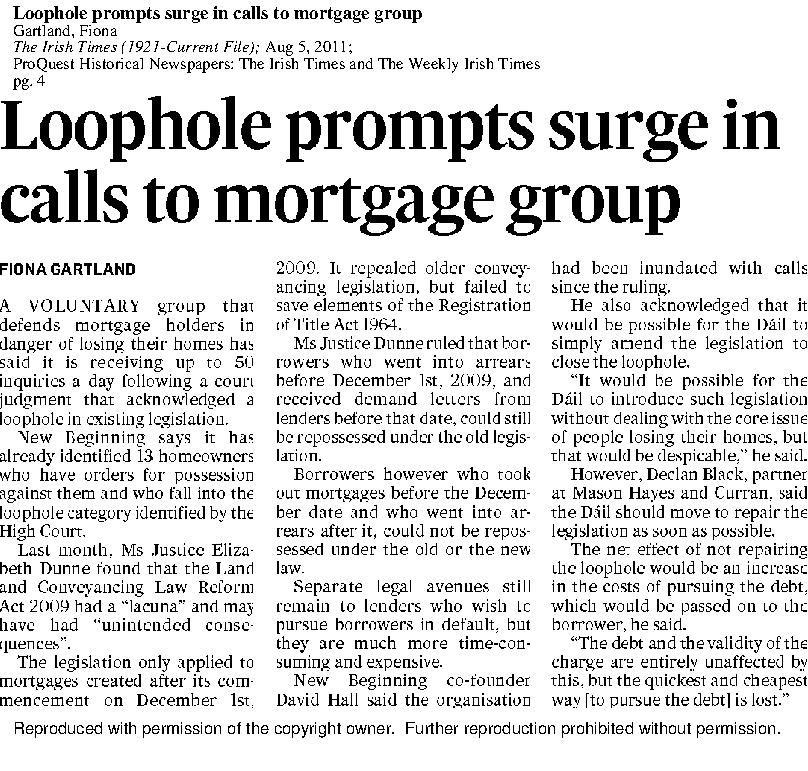
\includegraphics[width=0.49\linewidth]{loophole.pdf}
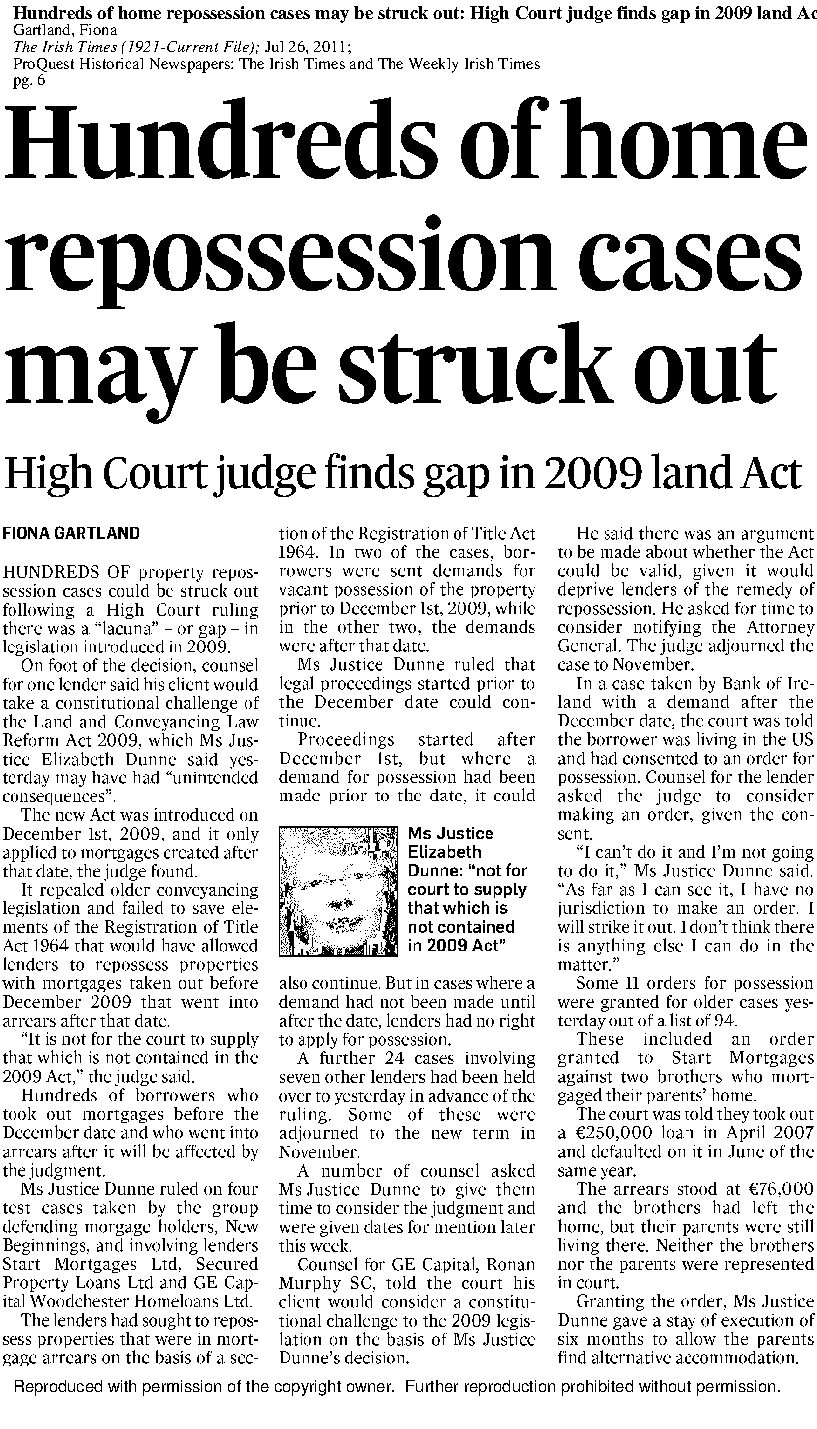
\includegraphics[width=0.49\linewidth]{july26.pdf}

\end{frame}

\begin{frame}{Research Design}

\begin{itemize}
\item
  Difference-in-difference variation created by the Dunne judgment
\item
  Diff 1: Pre-Post July 2011
\item
  Diff 2: Loans issued pre-post 1st December 2009
\end{itemize}

\(\implies\) For loans in a narrow window around 1st December 2009,
repossession risk is quasi-randomly removed unexpectedly on 25th July
2011

\end{frame}

\begin{frame}{Data}

\begin{itemize}
\item
  Loan-level data on Irish mortgages issued 180-days either side of the
  cutoff: 1st December 2009
\item
  Quarterly panel data on default, balance, LTV, interest rate, rate
  type from Q3 2010- Q3 2012

  \begin{itemize}
  \tightlist
  \item
    origination information on income, age, vintage
  \end{itemize}
\item
  Loans for home purchase (no equity release)
\item
  Treatment group: issued before 1st December 2009
\item
  Match loans across treatment control group on first period borrower
  age, location, income, interest rate, LTV-at-origination

  \begin{itemize}
  \tightlist
  \item
    Drop unmatched observations
  \end{itemize}
\item
  Roughly 8000 loans, half of which receive treatment in July 2011
\end{itemize}

\end{frame}

\begin{frame}{Default rates spiked for treated loans after Judgment}

\centering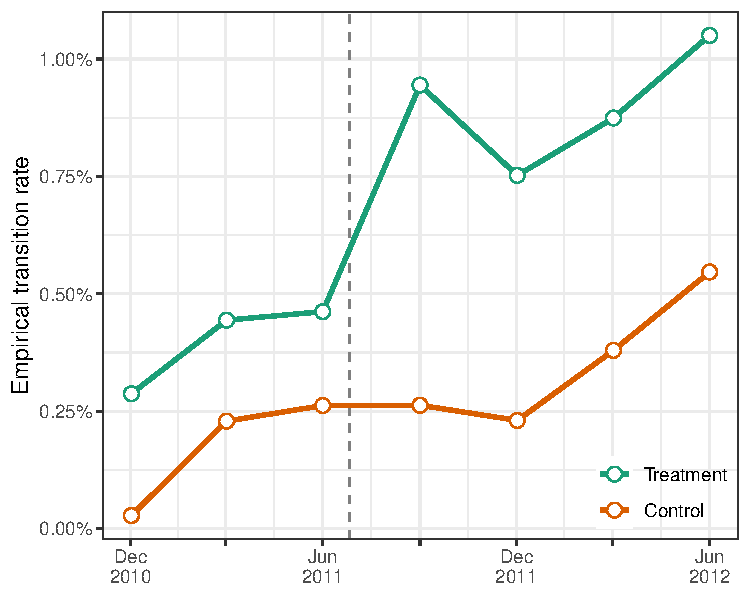
\includegraphics[width=0.75\linewidth]{transitions.pdf}

\end{frame}

\begin{frame}{Model}

\[ P(\textup{{default}}_{ijbgrt})=\alpha+\beta^{DD}(\textup{{Treatment}}_{j}\times\textup{Post}_{t})+\mathbf{X}_{it}^{\prime}\Psi+\phi_{rt}+\tau_{bgt}+\epsilon_{ijbgrt}\]

\begin{itemize}
\tightlist
\item
  Adjust for potential confounders:

  \begin{itemize}
  \tightlist
  \item
    Interest rates, interest rate types,
  \item
    LTV and negative equity
  \item
    Borrower region and age
  \item
    Vintage time trends
  \end{itemize}
\end{itemize}

\end{frame}

\begin{frame}{}

\centering
% Table created by stargazer v.5.2 by Marek Hlavac, Harvard University. E-mail: hlavac at fas.harvard.edu
% Date and time: Fri, Oct 06, 2017 - 20:00:14
\begin{tabular}{@{\extracolsep{5pt}}lccc} 
\\[-1.8ex]\hline 
\hline \\[-1.8ex] 
\\[-1.8ex] & \multicolumn{3}{c}{Default} \\ 
\\[-1.8ex] & (1) & (2) & (3)\\ 
\hline \\[-1.8ex] 
 Treatment & 0.002$^{***}$ & 0.0001 &  \\ 
  & (0.001) & (0.001) &  \\ 
  & & & \\ 
 Treatment$*$Post & 0.003$^{***}$ & 0.004$^{***}$ & 0.005$^{***}$ \\ 
  & (0.001) & (0.001) & (0.001) \\ 
  & & & \\ 
\hline \\[-1.8ex] 
Observations & 80,667 & 80,663 & 80,663 \\ 
\hline 
Time-varying controls & N & Y  & Y \\
Time FE & N & Y & -\\
Loan FE & N & N & Y \\
Region$*$RateType$*$Time FE& N & N & Y \\
\hline \\[-1.8ex] 
& \multicolumn{3}{r}{$^{*}$p$<$0.1; $^{**}$p$<$0.05; $^{***}$p$<$0.01} \\ 
\end{tabular} 


\end{frame}

\begin{frame}{Event study coefficients}

\centering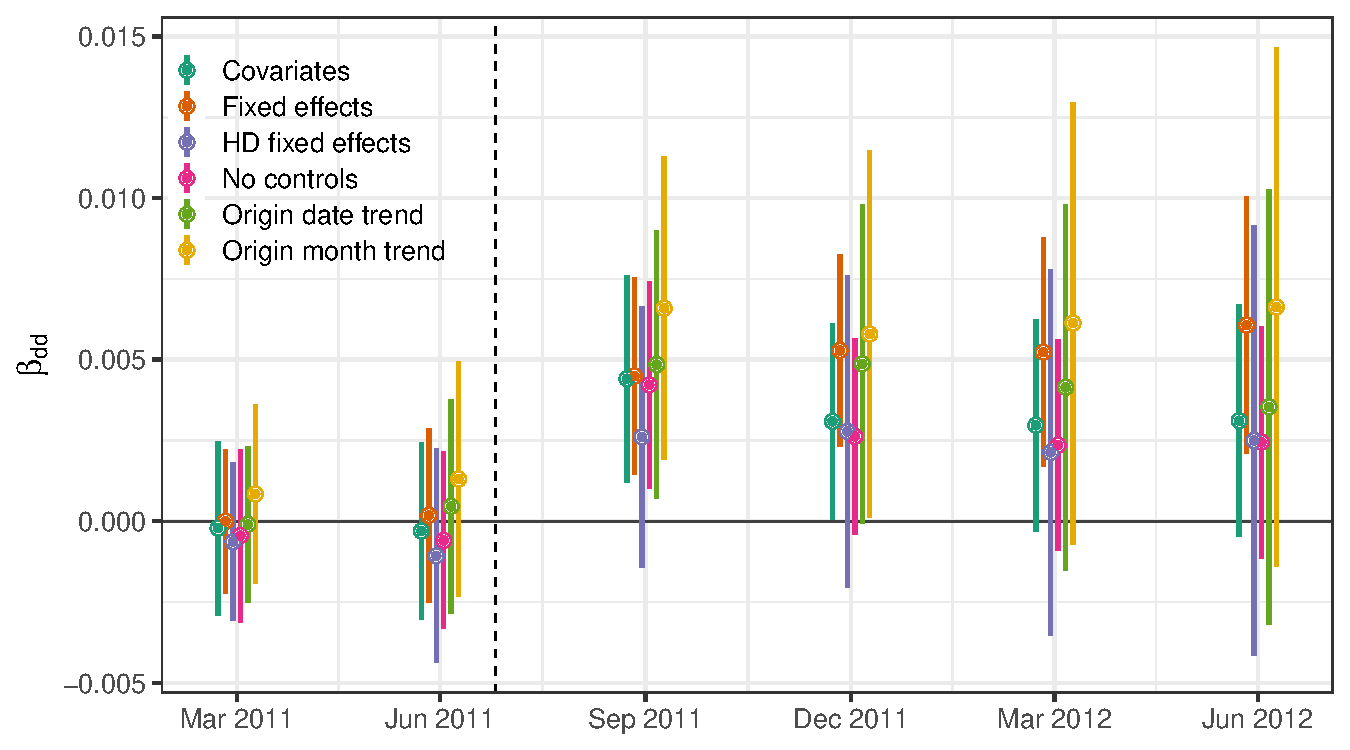
\includegraphics[width=\linewidth]{es_graph.pdf}

\end{frame}

\begin{frame}{Permutation Inference}

\begin{itemize}
\tightlist
\item
  Randomly choose other cut-off dates and repeat (X1000)
\end{itemize}

\centering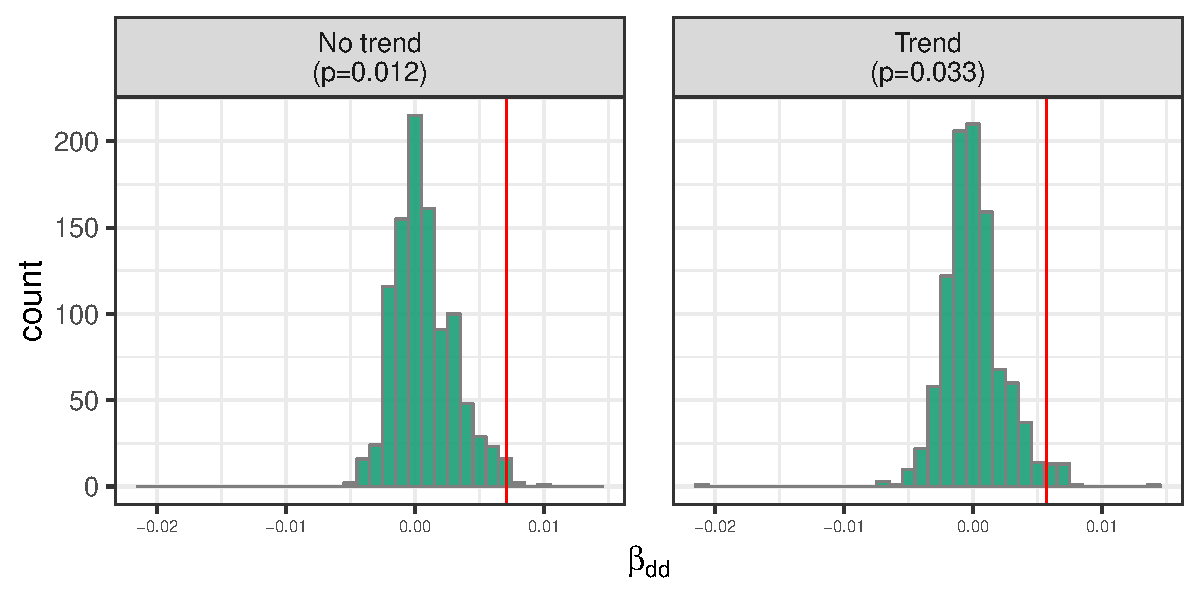
\includegraphics[width=\linewidth]{ri_plot.pdf}

\end{frame}

\begin{frame}{Mechanisms}

\begin{itemize}
\item
  Liquidity or strategic default?
\item
  Depending on which, policy implications are different
\item
  Incomplete insurance markets or imperfect mortgage contracts,
  liquidity default means high marginal utility borrowers getting
  payment relief
\item
  Strategic default: home no longer a good investment, can't even be
  repossessed so stop paying (pure moral hazard)
\end{itemize}

\end{frame}

\begin{frame}{Mechanisms}

\begin{itemize}
\tightlist
\item
  For a small sample (1347) loans, I can measure borrower's liquid
  account balance in 6-months prior to event

  \begin{itemize}
  \tightlist
  \item
    within same bank
  \end{itemize}
\item
  2 triple-diff regressions

  \begin{enumerate}
  \def\labelenumi{\arabic{enumi}.}
  \tightlist
  \item
    Terciles of liquid wealth distribution
  \item
    Terciles of loan-to-value distribution
  \end{enumerate}
\end{itemize}

\end{frame}

\begin{frame}{}

\begin{center}
\begin{tabular}{lrr}
\toprule
      & (1)   & (2) \\
\midrule
Treated $\times$ Post & -0.0046 & 0.015 \\
      & (0.372) & (0.005) \\
Treated $\times$ Post $\times$ LTV T2 & -0.0115 &  \\
      & (0.119) &  \\
Treated $\times$ Post $\times$ LTV T3 & 0.0198 &  \\
      & (0.008) &  \\
Treated $\times$ Post $\times$ Account Balance T2 &       & -0.0102 \\
      &       & (0.171) \\
Treated $\times$ Post $\times$ Account Balance T3 &       & -0.0166 \\
      &       & (0.026) \\
      \midrule
 {\it Obs}     & 7998  & 7998 \\
\bottomrule
\end{tabular}
\end{center}

\end{frame}

\begin{frame}{Conclusion}

\begin{itemize}
\item
  Estimated treatment effect of removing repossession risk on default:
  0.3pp increase in quarterly default rate
\item
  Liquidity or moral hazard? Seems to be both

  \begin{itemize}
  \tightlist
  \item
    Effect driven by low liquid wealth borrowers
  \item
    Also by highest LTV borrowers
  \end{itemize}
\end{itemize}

\end{frame}

\end{document}
